\section{Ferramentas}
Essa sessão tem como objetivo explicar as ferramentas que serão utilizadas na implementação da pesquisa, e alem disso, introduzir alguns conceitos basicos sobre elas. É importante ressaltar que todo o projeto é \textit{Open Source}, conhecidos como projeto de código aberto, e todo o código criado para ele pode ser encontrado na plataforma de versionamento do GitHub\footnote{\url{https://github.com/getdumont}}.

A pesquisa inicialmente foi projetada para rodar totalmente na nuvem e utilizando alguns recursos pagos, porem, ela será detalhada para ser implementada de forma gratuita. É possível localizar no anexo 1, as alterações necessárias e o projeto original seja implementado. Usamos basicamente 6 ferramentas durante todo o processo: Git, Docker, Mongo, Twitter, Google e Amazon. Contudo, a Amazon seria apenas utilizada para caso de subir todo o sistema para nuvem, logo essa sessão ira tratar unicamente das 5 primeiras ferramentas citadas. Como dito o código do projeto é aberto e por mais que não seja explicado o funcionamento do Git de maneira abrangente e complexa o detalhamento começara pela ferramenta.

\subsection{Git e Github}
O Git é uma ferramenta de versionamento de código, ou seja, uma ferramenta utilizada para que toda a alteração que alguém fizer em um código tenha a possibilidade de ser marcada, assim criando uma arvore das modificações e dando ao usuário a possibilidade de navegar entre suas alterações. A ferramenta foi criada por Linus Torvalds durante a criação de Linux, para que fosse possível manter um histórico seguro do desenvolvimento do sistema operacional. Entretanto, o Git é unicamente uma ferramenta de terminal, com o desenvolvimento da internet e os recursos gráficos sendo cada vez mais utilizados para representações, juntamente com a necessidade de algo mais acessível, nasceram varias interfaces para a ferramenta, uma delas e também a maior, o GitHub ganhou tração e é hoje uma das maiores plataformas de código aberta do mundo e recentemente foi adquirida pela Microsoft\footnote{\url{https://g1.globo.com/economia/tecnologia/noticia/microsoft-compra-github-por-us-75-bilhoes.ghtml}}.

É importante saber sobre Git nos dias de hoje, se quiser descobrir mais é possível achar todo o necessário em um livro\footnote{\url{https://git-scm.com/book/en/v2}} fornecido pela própria mantenedora da ferramenta. No caso desse trabalho é possível simplesmente baixar o código pelo Github. Para isso, vamos entender a interface do GitHub.

Se observar a figura \ref{fig:git_init}, pode-se notar um cabeçalho com alguns menus, logo abaixo o nome da organização getdumont seguida pelo nome do repositório\footnote{Repositório é o nome dado ao local onde ficará armazenado todo o código de um determinado projeto}. Então pode-se notar 5 abas, que nesse momento são irrelevantes, seguindo encontra-se alguns dados como descrição, algumas estatísticas e por fim o botão verde \textit{Clone or Download}, aqui pode-se baixar o código clicando no botão e em seguida clicando em \textit{Download ZIP}. Além disso, logo abaixo é possível ver uma tabela com a estrutura do projeto, essa estrutura é navegável pelo browser, assim qualquer arquivo citado durante essa documentação pode ser acessado sem necessidade do código na maquina.

\begin{figure}
    \centering
    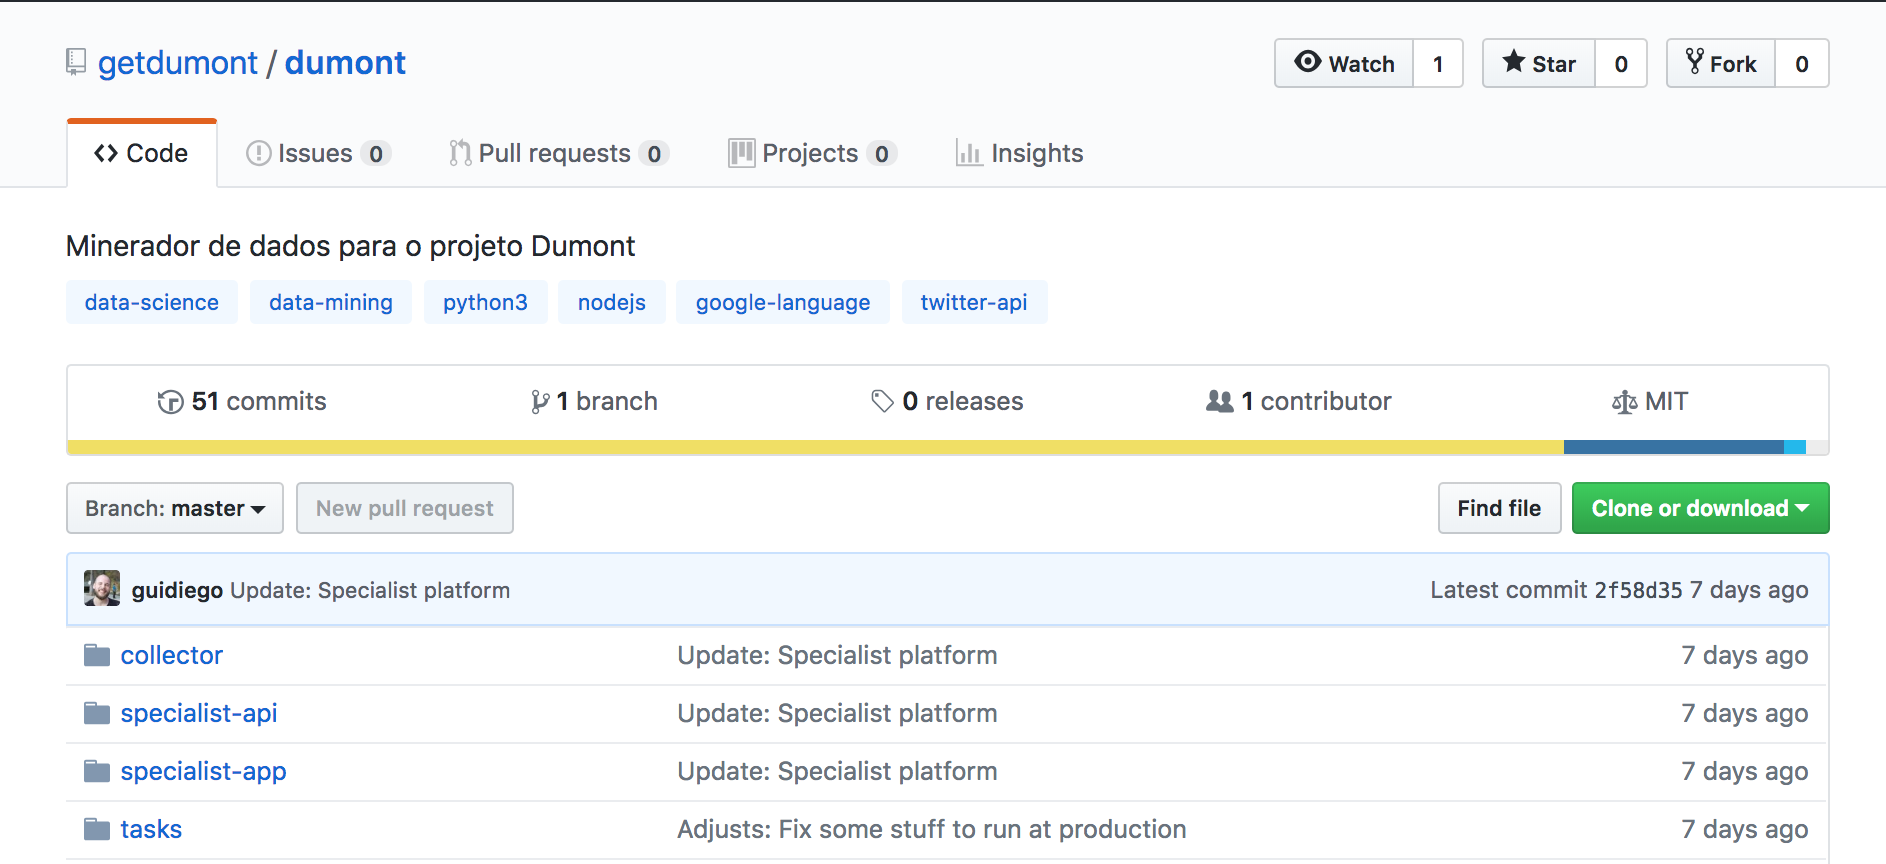
\includegraphics[width=.8\textwidth]{imagens/git_init.png}
    \caption{Imagem demonstrando a interface inicial do git}
    \label{fig:git_init}
\end{figure}

Já na figura \label{fig:git_file}, pode-se observar um exemplo do que foi dito anteriormente. Aqui uma demonstração de como fica um dos arquivos do projeto aberto no navegador. As 2 coisas mais importantes a serem notadas aqui é o caminho do arquivo \textit{dumont/collector/index.js} e as linhas que são mostradas no arquivo. Será utilizado destes recursos durante a documentação para exemplificar e apontar códigos.

\begin{figure}
    \centering
    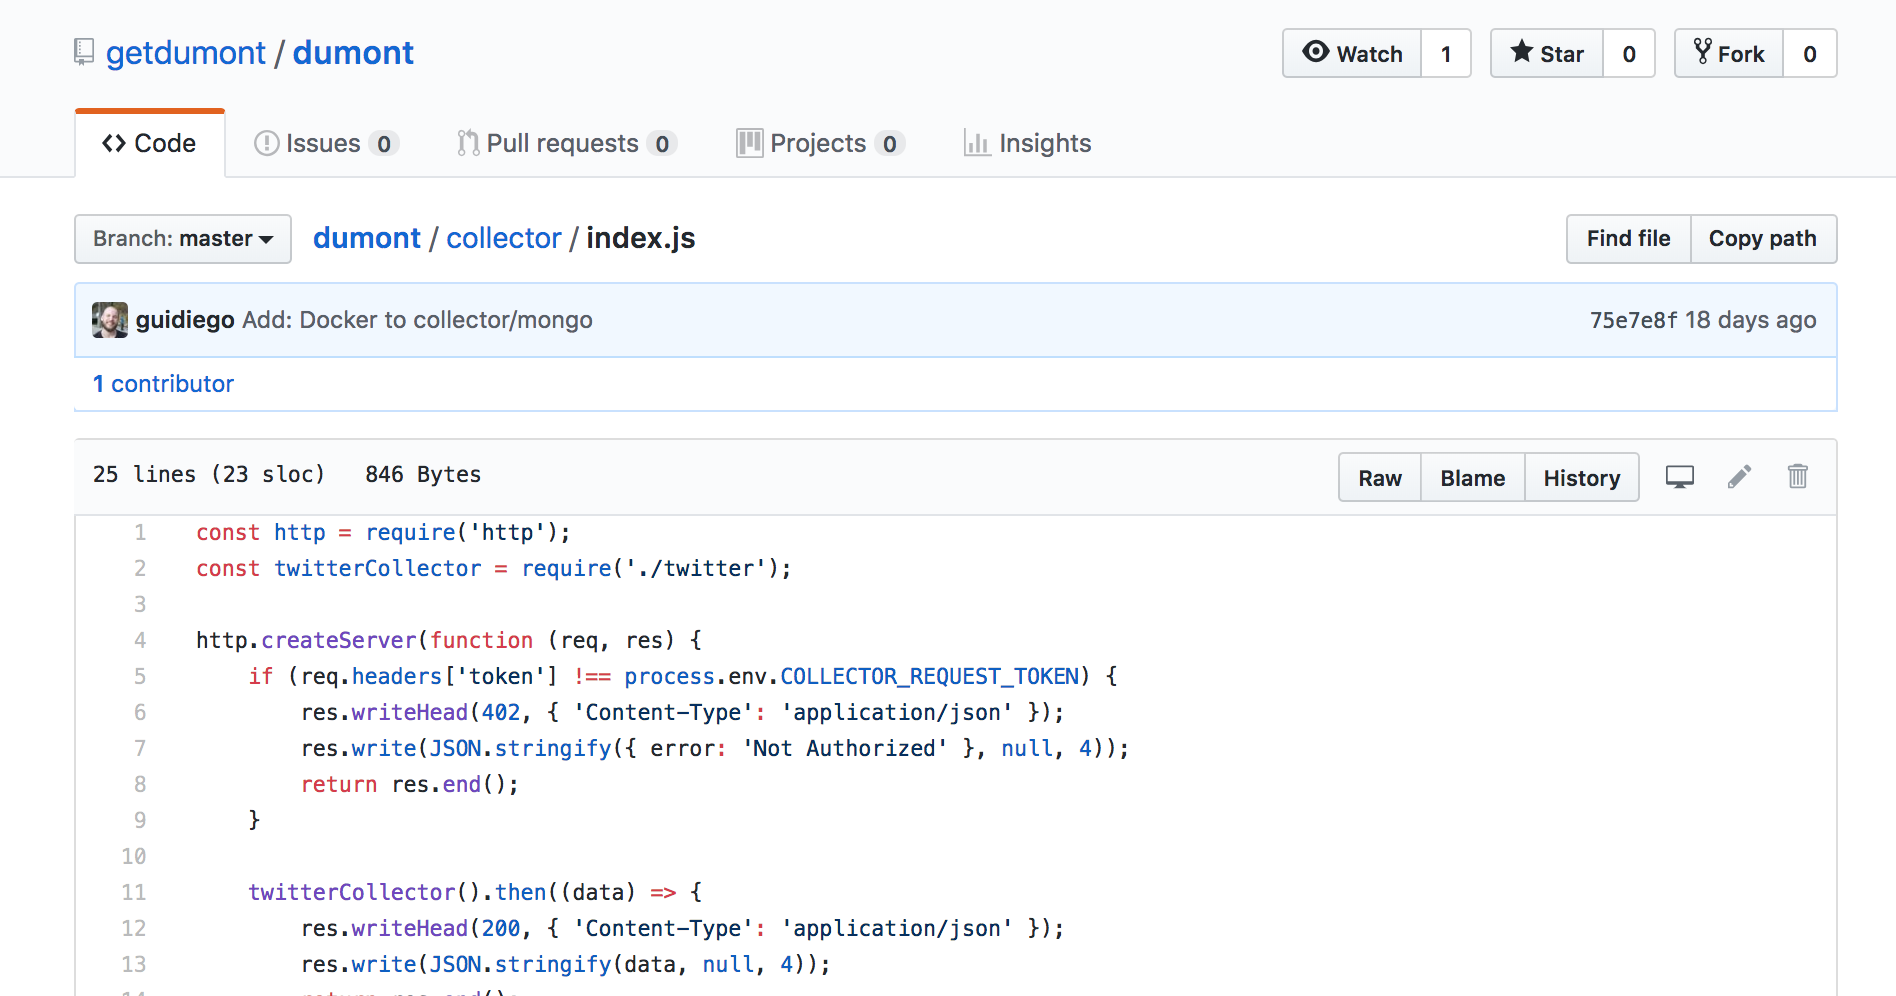
\includegraphics[width=.8\textwidth]{imagens/git_file.png}
    \caption{Imagem demonstrando a interface do git referente a um arquivo do projeto}
    \label{fig:git_file}
\end{figure}

Introduzido o Github, e tendo o código na máquina (caso haja a necessidade de reprodução desse projeto), é possível realizar os próximos passos. A próxima parte mais relevante nesse processo é entende como funciona o Docker.

\chapter{Docker}
\label{app:docker}

A modernidade e o avanço na programação levaram os desenvolvedores a publicarem suas aplicações cada vez mais rápido e com maior frequência. Com o tempo se criou o termo DevOps, a abreviação para o que em português seria: “Desenvolvimento e Operação”. Usualmente os times de DevOps eram compostos pelos indivíduos responsáveis por operacionalizar toda a parte de publicação e monitoramento das aplicações. As dificuldades encontradas por times era, e até hoje ainda é, a divergência entre tecnologia perante diferentes ambientes, e principalmente, o tempo que a aplicação demora em seu \textit{Deploy} e \textit{Rollback}\footnote{\textit{Deploy} é o termo utilizado para publicar algo na nuvem, enquanto \textit{rollback} é o termo para retroceder uma versão recém publicada}.

O Docker nasceu para suprir não só esse problema, padronizando ambientes, mas também para isolar as dependências e ferramentas instaladas através dele. Uma vez executado o Docker cria o que chamamos de imagem, é basicamente uma versão minimalista do Linux que tem todas as dependências e códigos da sua aplicação. Com essa imagem gerada é possível executa-la e dar origem a um \textit{container}. Podem existir vários containers rodando simultaneamente, e o mais importante, interligados. Com isso subir um banco de dados especifico sem instala-lo em sua maquina, ou testar sua aplicação com outras versões de uma linguagem, se tornou algo simples. O Docker fez tanto sucesso que as principais fornecedoras de aplicação em nuvem como a Amazon, Google e Azure tem serviços dedicados a rodarem a partir da ferramenta.

Para facilitar a execução, foram configuradas todas as imagens necessárias para que a execução seja rápida e direta. Obviamente coordenar uma grande leva de containers seria um problema, para isso, foi criado o Docker Compose, basicamente um arquivo que administra todas as imagens e interliga elas tornando assim mais fácil a conexão entre os containers. Dentro da raiz do projeto existe um \textit{dumont/docker-compose.yml}, com todas as partes da aplicação. Existe também um \textit{dumont/docker-compose.dev.yml} que é o que será utilizado para rodar a pesquisa na máquina local.

Para baixar a ferramenta basta acessar o site\footnote{\url{https://www.docker.com/products/docker-desktop}} e baixa-la para seu sistema operacional. Uma vez com o Docker e o código em mãos é necessário configurar alguns outros elementos. Obviamente antes mesmo de coletar dados é necessário um lugar para guarda-los, como já abordado utilizaremos o MongoDB.


\chapter{Instalando MongoDB}
O MongoDB é um banco não relacional, ou seja, um banco que não tem \textit{transactions}\footnote{Simboliza uma atividade realizada em um banco relacional} e é baseado inteiramente em documentos. Diferente de um banco não relacional, os dados inseridos nesse tipo de banco não tem uma normalização ou qualquer tipo de padrão. No caso do Mongo a unica identificação utilizada para interligar os documentos é a nomeada Coleção\footnote{As Coleções servem para agrupar tipos especificos de documentos.}.

A maior facilidade e vantagem do mongo é exatamente que em caso de alteração na estrutura dos dados não é necessária uma migração formal para normalizar os dados no banco para a nova estrutura. Normalmente todo o dado do mongo é tratado pela aplicação utilizando, caso necessário, bibliotecas que validam o dado antes de inseri-lo no banco. Alem de nesse trabalho os atributos mudarem conforme forem localizadas novas formas de explorar e aprender com o dado, outro ponto importante é que serão realizadas várias consultas para ler os dados, o que nos leva a outra vantagem do banco não relacional: a leitura é mais rapida uma vez que é basicamente texto sendo indexado em coleções.

Dentro do trabalho existem algumas estruturas mais fechadas e outras que irão variar mais com o passar do desenvolvimento, pode-se notar na figura \ref{fig:entities}, a visão inicial do que seria a estrutura de nossos documentos. Teremos duas coleções mais relevantes \textit{Tweet} e \textit{User} aqui ficaram armazenados os dados do Twitter, as demais estruturas são estruturas periféricas criadas para suportar o sistema de armazenamento de dados especialistas. Para isso existem duas estruturas \textit{Answer} e \textit{Word} que servem para que os especilistas inserirem palavras chaves de um determinado tweet, juntamente com a possibilidade de um mapeamento do mesmo dentro de algum dos items da EADS. Por final existem mais duas coleções a \textit{Specialist} que armazena os especialistas registrados no nosso sistema e o \textit{List} que é uma coleção auxiliar para agrupar uma quantidade de tweets tornando mais facil para nossa aplicação apresenta-los aos especialista e coletar analise.

\begin{figure}
    \centering
    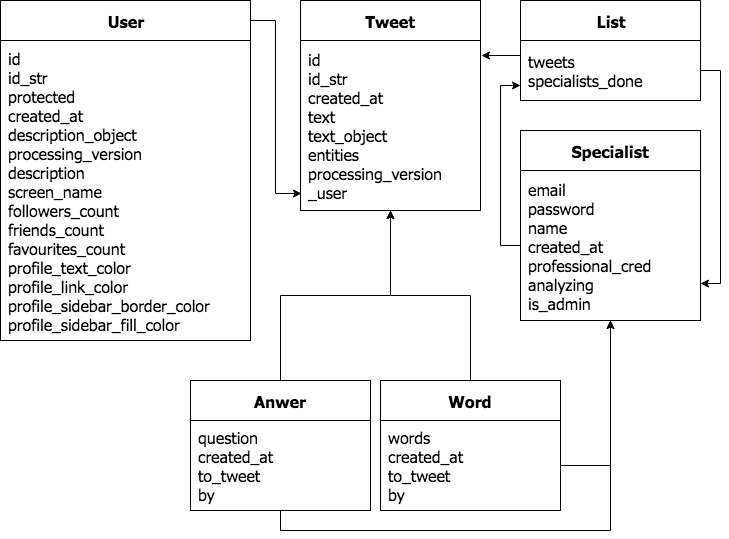
\includegraphics[width=.8\textwidth]{imagens/entities.png}
    \caption{Mapa de entidades do projeto}
    \label{fig:entities}
\end{figure}

Como dito anteriormente, o Docker ja foi préviamente configurado, e assim que você rodar qualquer um dos serviços o mongo local ja estara pronto para receber dados. Entretando, se existir a intenção de subir a pesquisa publicamente, no anexo pode-se encontrar um pequeno adendo de como configurar um mongo gratuito utilizando a plataforma Atlas. Outra ferramenta relevante é o Robo3T\footnote{\url{https://robomongo.org/download}} uma interface gráfica para explorar seu banco, você pode baixa-la caso queira olhar os dados antes dele ser condensado em um dataset menor.

Para que o coletor funcione e insira dados no mongo é necessário configurar as apis do Twitter e a do Google Language.
\chapter{Configurando APIs}
Dentro do projeto é utilizado as apis do Twitter e do Google Language, nessa parte será detalhado um pouco mais sobre as APIs e também como configura-las. Já foi abordado alguns aspectos técnicos na revisão, logo, esse detalhamento será voltado a parte de implementação.

A coleta será feita utilizando a API publica do twitter, o link para a documentação é \url{https://developer.twitter.com/en/docs}. Será trabalhado no projeto duas entidades: Tweet e Usuário. O tweet é a entidade que representa a publicação do usuário, enquanto o usuário contém informações necessárias sobre o seu perfil.

Para que seja possível acessar a API é necessário criar uma conta de desenvolvimento e gerar o \textit{token} de acesso\footnote{\url{https://apps.twitter.com/app/new}}. Com a chave em mãos é possível replicar o arquivo /dumont/sample\_env dentro do projeto Dumont para dumont/dev.env, e conforme demonstrado na Figura \ref{fig:twitteropts}, completar os campos necessários.

\begin{figure}
    \centering
    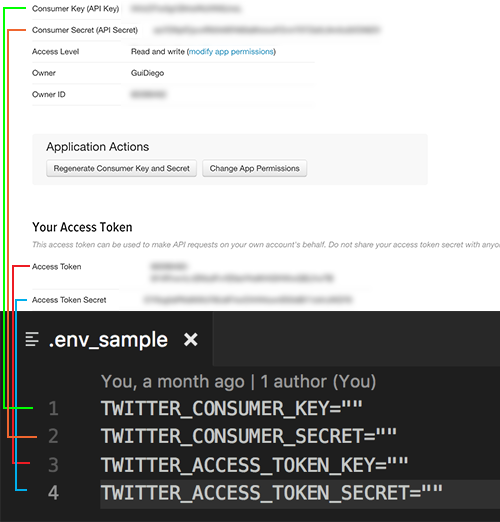
\includegraphics[width=.8\textwidth]{imagens/twitteropts.png}
    \caption{Imagem demonstrando onde cada chave deve ser inserida no código}
    \label{fig:twitteropts}
\end{figure}

Feito isso, é necessário conseguir o JSON de acesso do Google, esse arquivo serve como credencial para que seja possível obter os dados, Figura \ref{fig:twitteropts} pode-se observar que o valor \textit{GOOGLE\_APPLICATION\_CREDENTIALS} já esta definido como \textit{./google\_credentials.json}, ou seja, é necessário apenas baixar as credenciais, move-la para a pastas \textit{dumont/tasks} e renomear para \textit{google\_credentials.json}. Para conseguir acesso a essas credenciais acesse o site da api do Google Language\footnote{\url{https://cloud.google.com/natural-language/}} e clique em \textit{Try it Free}. Feito isso acontecera um redirecionamento para que seja escolhido uma conta google ou, em caso de nenhuma conta estiver previamente autenticada, a tela para efetuar a autenticação. Lembrando que é necessário para quem for replicar a pesquisa ter ao menos uma conta no google (pode ser o mesmo e-mail do gmail). Após selecionado será redirecionado para uma tela informando que o usuário tem 300 dólares gratuitos dentro da google cloud. O primeiro aceite é para receber notificações dos serviços da Google, e pode ficar marcado como "não". O segundo é o aceite dos termos de uso, e esse tem que estar marcado como "sim". Após isso basta clicar em "Agree and Continue". Basta completar algumas informações e informar um cartão de crédito valido (lembrando que isso é apenas um passo de segurança para a google). Feito isso você será direcionado para um \textit{dashboard} da google cloud, como mostrado na figura \ref{fig:googleflow}, basta clicar em \textit{Api \& Services > Credentials}, logo após acessar a tela de credenciais clique em \textit{Create credentials > Service Account Key} após mais um redirecionamento selecione o Serviço (caso não tenha um ainda, basta criar clicando em \textit{New service account}), mantenha a opção JSON marcada e clique em \textit{create}. Logo que fizer isso um JSON com um nome aleatório será baixado em sua máquina, basta mover e renomear como já dito previamente.

\begin{figure}
    \centering
    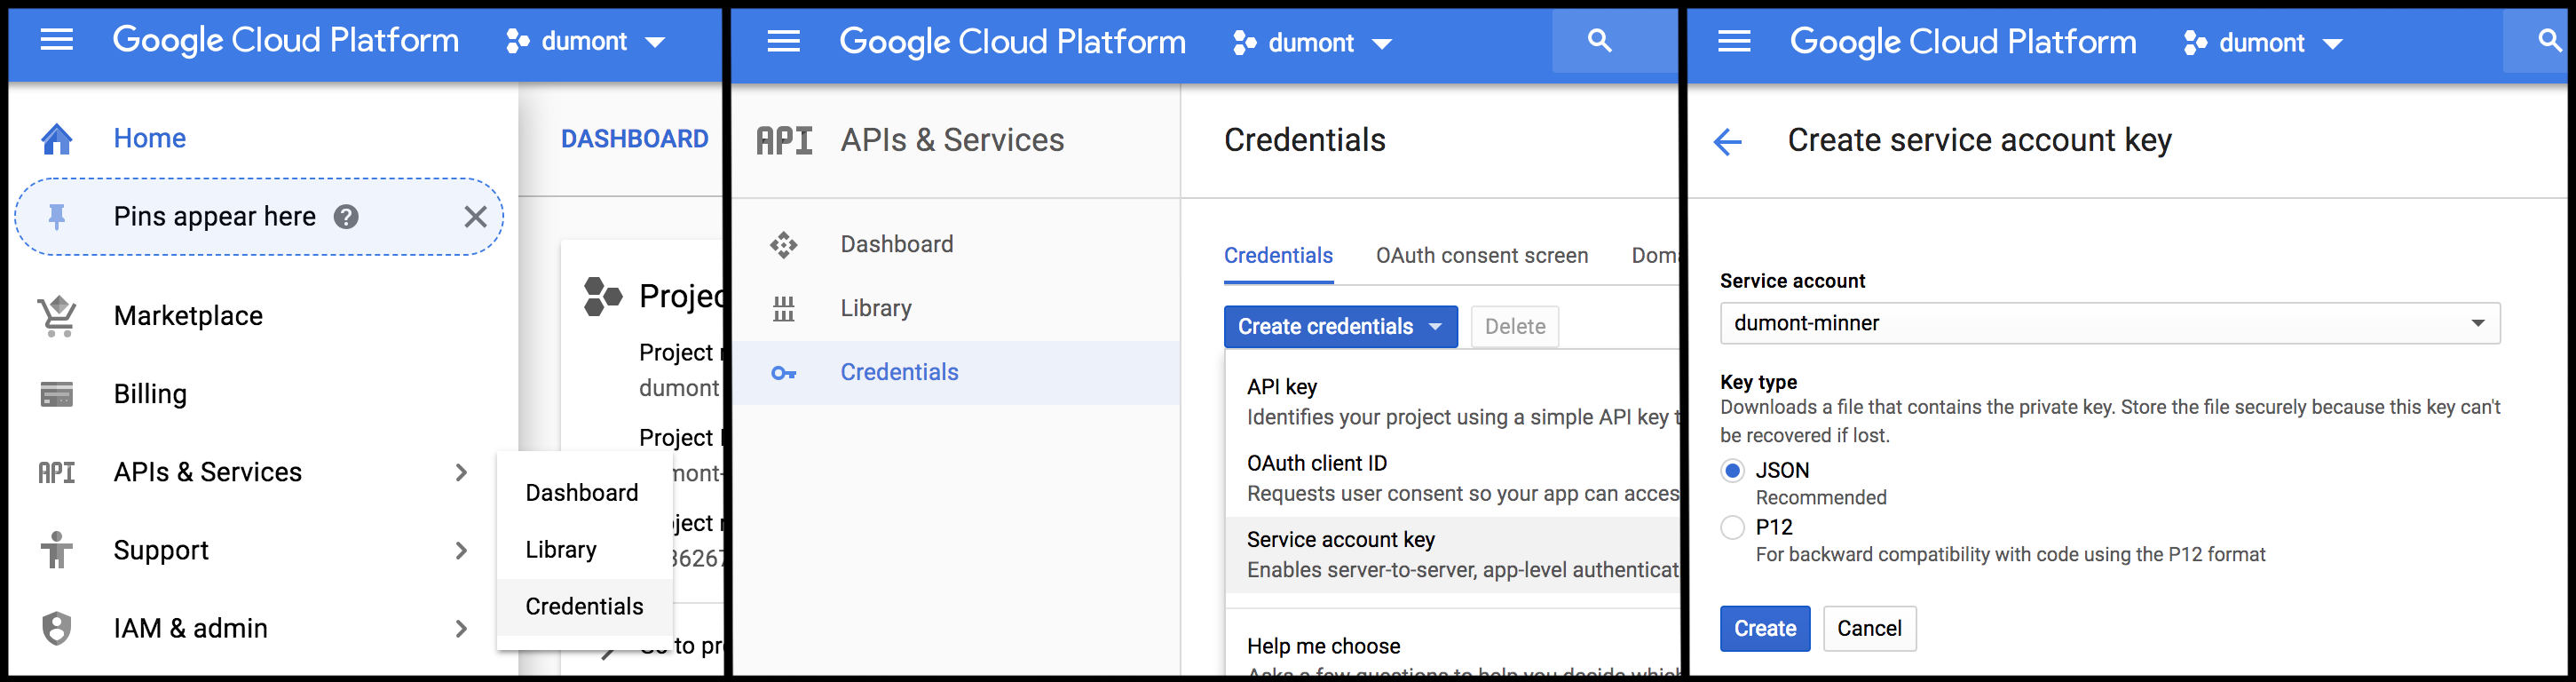
\includegraphics[width=1\textwidth]{imagens/googleflow.png}
    \caption{Imagem demonstrando passo a passo de como gerar o JSON de credencial}
    \label{fig:googleflow}
\end{figure}

Agora é possível executar os comandos, entretanto, existem configurações que devem ser retiradas e/ou alteradas para evitar problemas. Para isso vamos entrar na parte que envolve os processos de coleta e mineração de dados, com o intuito de entender as ultimas configurações e como todo o processo é executado.

